% !TEX encoding = UTF-8 Unicode
% © J.Roussel 2017-10-10
% !TEX root = ${file}
\documentclass[border=2pt]{standalone}
\usepackage{tikz}
\begin{document}
%-------------------------------------------
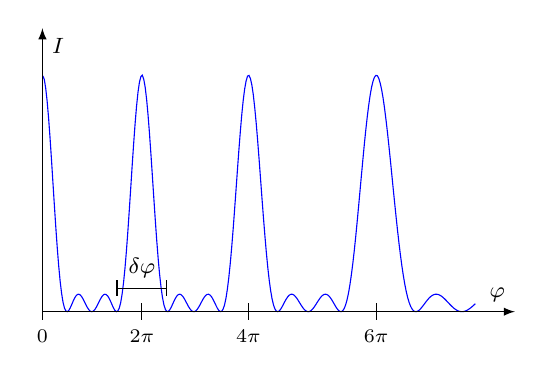
\begin{tikzpicture} [xscale=5,yscale=3]
	\def \N {4}%nombre de fentes
	\def \NN {8}%nombre de fentes
	\def \al {4}%a/lambda
	% legende
	\draw[shift={({pi*asin((0/2)/\al)/180},0)}] (0pt,1pt) -- (0pt,-1pt) node[below] {\scriptsize $0$};
	\foreach \x in {2,4,6}{
		\draw[shift={({pi*asin((\x/2)/\al)/180},0)}] (0pt,1pt) -- (0pt,-1pt) node[below] {\scriptsize $\x\pi$};
		}
		%graphe
		\draw [blue,domain=0.001:1.1,samples=300] plot (\x,{(sin(pi*\N*\al*sin(\x r) r)/(\N*sin(pi*\al*sin(\x r) r)))^2});
		\draw[->,>=latex] (0,0) -- (1.2,0) node[black,above left] {\footnotesize $\varphi$};
		\draw[->,>=latex] (0,0) -- (0,1.2) node[below right,black] {\footnotesize $I$};
		\draw[shift={({pi*asin(1/\al)/180},.1)},|-|] ({-1/(\N*(\al*\al-1)^.5)},0)--({1/(\N*sqrt(\al*\al-1))},0)node[midway,above]{\footnotesize $\delta\varphi$};
		% \draw (0.6,1.2)node{\footnotesize $N=\N$};
		% \begin{scope}[shift={(1.5,0)}]
		% 	% legende
		% 	\draw[shift={({pi*asin((0/2)/\al)/180},0)}] (0pt,1pt) -- (0pt,-1pt) node[below] {\scriptsize $0$};
		% 	\foreach \x in {2,4,6}{
		% 		\draw[shift={({pi*asin((\x/2)/\al)/180},0)}] (0pt,1pt) -- (0pt,-1pt) node[below] {\scriptsize $\x\pi$};
		% 		}
		% 		%graphe
		% 		\draw [blue,domain=0.001:1.1,samples=500] plot (\x,{(sin(pi*\NN*\al*sin(\x r) r)/(\NN*sin(pi*\al*sin(\x r) r)))^2});
		% 	\draw[->,>=latex] (0,0) -- (1.2,0) node[black,above left] {\footnotesize $\varphi$};
		% 	\draw[->,>=latex] (0,0) -- (0,1.2) node[below right,black] {\footnotesize $I$};
		% 	\draw[shift={({pi*asin(1/\al)/180},.1)},|-|] ({-1/(\NN*(\al*\al-1)^.5)},0)--({1/(\NN*sqrt(\al*\al-1))},0)node[midway,above]{\footnotesize $\delta\varphi$};
		% 	\draw (0.6,1.2)node{\footnotesize $N=\NN$};
		% \end{scope}
	\end{tikzpicture}	
\end{document}
